\documentclass[10pt,aspectratio=169]{beamer}
%设置为 Beamer 文档类型,设置字体为 10pt,长宽比为16:9
\usepackage{ccnu}			%导入 CCNU 模板宏包
\usepackage{amsmath,amsfonts,amssymb,bm}   %导入数学公式所需宏包
\usepackage{color}			 %字体颜色支持
\usepackage{graphicx,hyperref,url}
 %\usepackage{CJK}
\usepackage{multirow,booktabs}
\newcommand{\cu}{\boldsymbol}
\newcommand{\tabincell}[2]{\begin{tabular}{@{}#1@{}}#2\end{tabular}}  %表格内容强制换行
\beamertemplateballitem		%设置 Beamer 主题

\usepackage{algorithm,algorithmic}   %算法

\setbeamertemplate{caption}[numbered] %显示图、表的编号

\usepackage{fontspec}
\setsansfont{Times New Roman}  %设置字体
\usepackage{caption}  
%\usetheme{Madrid}  %beamer主题



%\usepackage{ctex} %可使用中文

%\CTEXoptions[today=old]  %日期显示为英文

\usepackage{wrapfig}

\title{Parallel and Distributed Computing in Statistics}

\author{Diao Tianbo}


\institute[CCNU]{
School of Mathematics and Statistics\\
Central China Normal University}

\date{\today}
\begin{document}
\begin{sloppypar}
	
	
\begin{frame}
\titlepage
\end{frame}				%生成标题页

\begin{frame}{Table of contents}
\tableofcontents
\end{frame}	             %生成目录页

\section{Introduction}
\begin{frame}[shrink]{Table of contents}
        \tableofcontents[sectionstyle=show/shaded,subsectionstyle=show/shaded/hide]
 \end{frame}

\begin{frame}{What is Parallel and Distributed Computing} \par
	{\bf {Wikipedia}}
\begin{itemize}
	
	\item {\color{red}Parallel computing\footnote{Parallel computing:https://en.wikipedia.iwiki.eu.org/wiki/Parallel\_computing}}: Parallel computing is a type of computation where 	many calculations or the execution of processes are carried out simultaneously.
		\item {\color{red}Distributed computing\footnote{Distributed computing:https://en.wikipedia.iwiki.eu.org/wiki/Distributed\_computing}}:  A distributed system is a system whose components are located on different networked computers, which communicate and coordinate their actions by passing messages to one another from any system.
\end{itemize}
\end{frame}	

\begin{frame}{What is parallel and distributed computing}   \par
	{\bf {Common Explanation}}
	\begin{itemize}
		\item {\color{blue}Parallel computing}: Multiple processors performs multiple tasks assigned to them simultaneously. Memory in parallel systems can either be shared or distributed. 
		\item {\color{blue}Distributed computing}: Each processor has its own private memory (distributed memory). Information is exchanged by passing messages between the processors.
	\end{itemize} 
	\begin{figure}
		\centering
		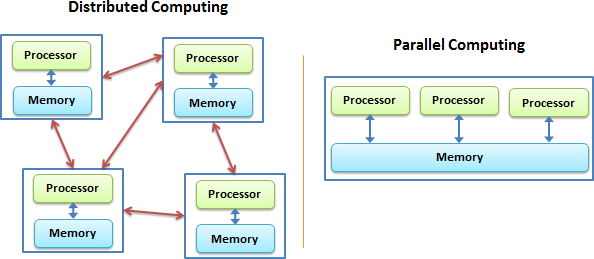
\includegraphics[width=8cm]{picture//1} 
		\caption{The difference between parallel and distributed computing}
	\end{figure}
\end{frame}

\begin{frame}{The difference}  \par
	{\bf{Difference between Parallel Computing and Distributed Computing:}}
	\begin{table}
		\caption{Comparison}
		\resizebox{\textwidth}{!}{
			\begin{tabular}{l|l}
				\hline
				\centerline{Parallel Computing} & \centerline{Distributed Computing}  \\
				\hline
				1.Many operations are performed simultaneously & System components are located at different locations  \\
				2.Single computer is required & Uses multiple computers  \\
				3.Multiple processors perform multiple operations & Multiple computers perform multiple operations  \\
				4.It may have shared or distributed memory & It have only distributed memory  \\
				5.Processors communicate with each other through bus & Computer communicate with each other through message passing  \\
				6.Improves the system performance &Improves system scalability, fault tolerance and resource sharing capabilities  \\
				\hline
			\end{tabular}
		}
	\end{table}
\end{frame}

\begin{frame}{Why we need parallel and distributed computing}  
	\begin{itemize}
		\item {\color{blue}Data World}: Big data is ubiquitous today. In the era of “big data,” in many applications, it is impossible to store data in a single device or central location.
		\item {\color{blue}New Challenge}: The big data challenges current numeric statistical and	machine learning methods, visualization methods, computational methods and computational environments.  
	\end{itemize} 
\begin{figure}[htbp]
	\centering
	\begin{minipage}[t]{0.48\textwidth}
		\centering
		
\includegraphics[width=5cm]{picture//2}
		\caption{Are we drowning in a sea of Big Data}
	\end{minipage}
	\begin{minipage}[t]{0.48\textwidth}
		\centering
		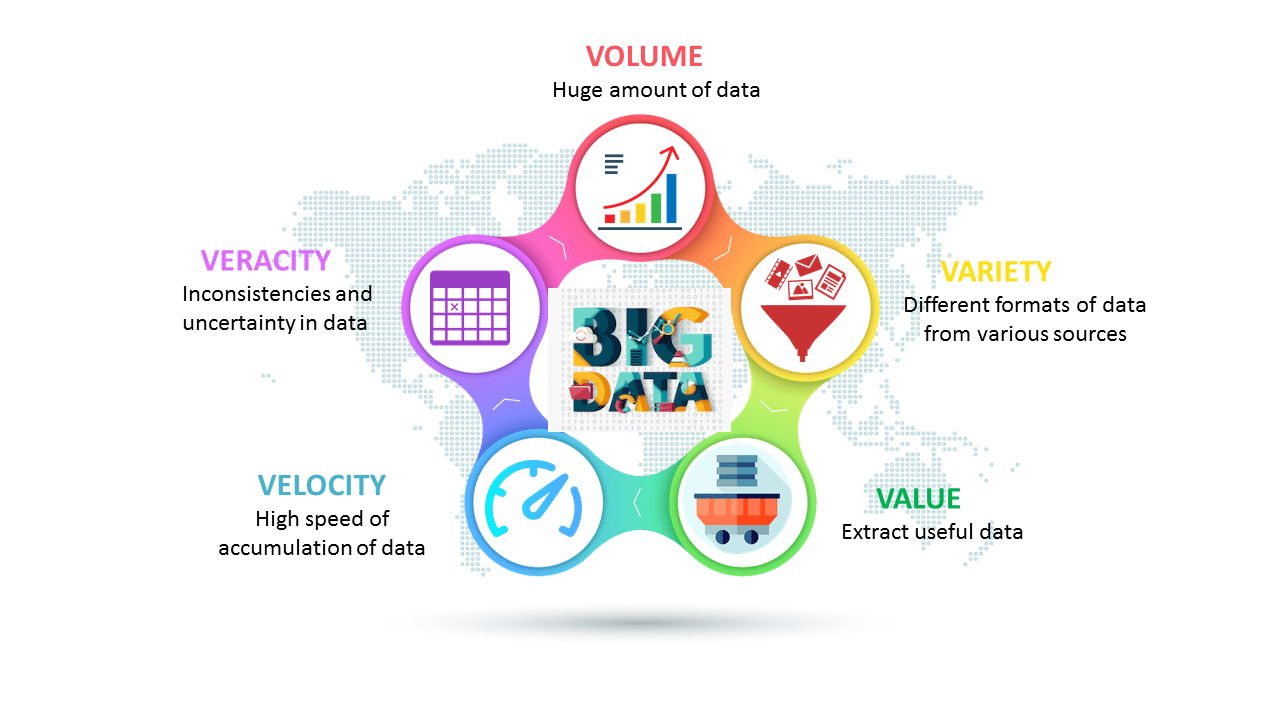
\includegraphics[width=6cm]{picture//3}
		\caption{Features of Big Data}
	\end{minipage}
\end{figure}
\end{frame}


\section{Parallel Computing}
\subsection{History and its development}
\begin{frame}[shrink]{Table of contents}
        \tableofcontents[sectionstyle=show/shaded,subsectionstyle=show/shaded/hide]
 \end{frame}



\begin{frame}{History and its development}
		\begin{columns}      %%分栏
			\column{.5\textwidth}
				\begin{itemize}
					\item Flynn (1966; 1972) created one of the earliest classification systems for parallel (and sequential) computers and programs, known as {\bf{Flynn's taxonomy}}.
					\item single-instruction-single-data({\bf{SISD}})
					\item single-instruction-multiple-data({\bf{SIMD}})
					\item Multiple-instruction-single-data({\bf{MISD}})
					\item Multiple-instruction-multiple-data({\bf{MIMD}})
				\end{itemize}
	
			\column{.5\textwidth}
				\begin{figure}
					\centering
					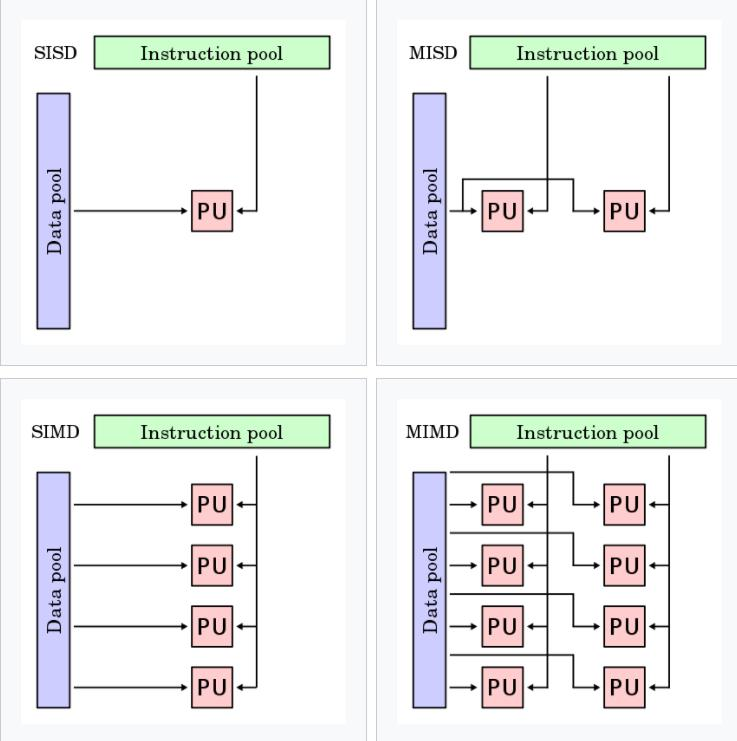
\includegraphics[width=5cm]{picture//4} 
					\caption{Flynn's taxonomy}
				\end{figure}
			
	\end{columns}
\end{frame}


\begin{frame}{History and its development} \par
{\bf{Amdahl's law:}}
In parallel statistical computing, the speed-up for $r$ processors is defined as $S_r=\frac{T_1}{T_r}$, where $T_k$ is the running time with $k$ processors. According to Amdahl’s law, the theoretical limit of speed-up is
\begin{equation}
S_r \leq \frac{1}{(1-\alpha)+\frac{\alpha}{r}}\leq r   \nonumber
\end{equation} 
where $\alpha$ is the proportion of the computation that can be run in parallel, and $1-\alpha$ is the proportion that remains serial.
\end{frame}


\begin{frame}{History and its development}
	\begin{columns}      %%分栏
		\column{.5\textwidth}
		\begin{itemize}
			\item {\bf{Amdahl's law:}}
		 \begin{equation}
			S_r \leq \frac{1}{(1-\alpha)+\frac{\alpha}{r}}\leq r   \nonumber
			\end{equation} 
			\item $S_r$ is the speed-up for $r$ processors
			\item where $\alpha$ is the proportion of the computation that can be run in parallel
		\end{itemize}
		
		\column{.5\textwidth}
		\begin{figure}
			\centering
			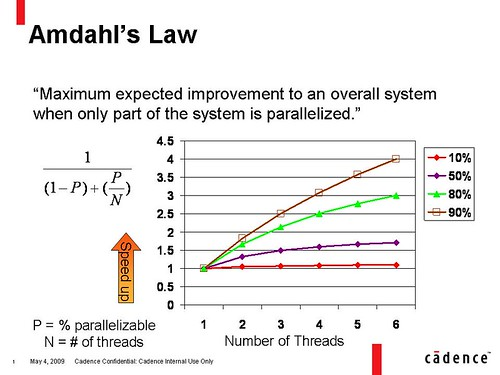
\includegraphics[width=7cm]{picture//5} 
			\caption{Amdahl's law}
		\end{figure}
		
	\end{columns}
\end{frame}



\begin{frame}{History and its development} \par
{\color{blue}{Parallel processing for statistics: a review}}
\begin{itemize}
	\item {\bf{Exploiting parallelism for statistics is not a new idea, nor
			is it entirely ignored in major statistical texts.}}
	\item Chambers (1977) mentioned the use of parallel computing in data analysis situations where the magnitude of	computation makes interactive analysis impossible.
	\item Thisted (1988) briefly mentioned parallel computers as
	being an ideal method of implementing Jacobi methods
	for extracting eigenvalues. 
	\item Schervish (1988) considered a variety of parallel applications-including discrete-finite inference, a computerintensive approach for the analysis of discrete data-where
	the dominant aspect of the computation is simple summation
	of large sets of data.\\	
		(to be continued)
\end{itemize}
\end{frame}

\begin{frame}{History and its development} \par
	{\color{blue}{Parallel processing for statistics: a review}}
	\begin{itemize}
		\item Skvoretz et al. (1992) employed an NCUBE/10 hypercube
		multiprocessor (MIMD) to assess the application of parallel
		processing to typical large-scale social science research.
		\item Schmidberger (2009) gave a classification of parallel statistical computers:	multicore system,multiprocessor system,multicomputer with computing cluster(distributed computer), and multicomputer with grid computing (grid computers). 
		\item The classification is	also very popular in parallel computers. The tutorial of Creel and Goffe (2008) urged further use of these techniques by economists. Creel (2005) identified a steep learning curve and
		expensive hardware as the main barriers to adoption.					
	\end{itemize}
\end{frame}

\section{Distributed Computing}
\subsection{A Overview of Distributed Computing}
\begin{frame}[shrink]{Table of contents}
	\tableofcontents[sectionstyle=show/shaded,subsectionstyle=show/shaded/hide]
\end{frame}

\begin{frame}{A Overview of Distributed Computing}
	\begin{itemize}
		\item The study of distributed computing became its own branch of computer science in the late 1970s and early 1980s. 
		\item The first conference in the field, Symposium on Principles of Distributed Computing (PODC), dates back to 1982, and its counterpart International Symposium on Distributed Computing (DISC) was first held in
		Ottawa in 1985 as the International Workshop on Distributed Algorithms on Graphs.
	\end{itemize}
\end{frame}

\begin{frame}{A Overview of Distributed Computing} \par
{\bf{Distributed Architectures:}}
	\begin{itemize}
		\item Various hardware and software architectures are used for distributed computing.  
		\item At a lower level, it is
		necessary to interconnect multiple CPUs with some sort of network, regardless of whether that network is
		printed onto a circuit board or made up of loosely coupled devices and cables.
		\item At a higher level, it is necessary
		to interconnect processes running on those CPUs with some sort of communication system.
	\end{itemize}
\end{frame}

\begin{frame}{A Overview of Distributed Computing} \par
	{\bf{Distributed Computing in Statistics:}}
\begin{columns}      %%分栏
		\column{.5\textwidth}
		\begin{itemize}
			\item With the advent of the Big Data era, distributed computing is ushering in its own spring of development in statistics. \\
			In recent years, more and more statistical papers on the processing of data are distributed. 
			\item {\bf{Distributed computing is already one of the mainstream of statistics}} 
				\end{itemize}
	\column{.5\textwidth}
		\begin{figure}
			\centering
			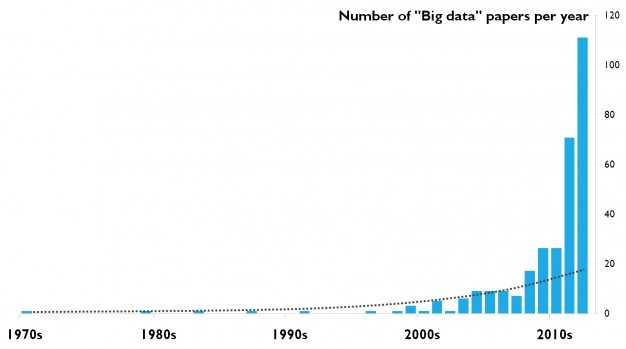
\includegraphics[width=7cm]{picture//6} 
			\caption{Fast Growing Distributed Statistics Essays}
		\end{figure}
	\end{columns} 
\end{frame}
	
\subsection{Example for Distributed Computing}  
\begin{frame}[shrink]{Table of contents}
        \tableofcontents[sectionstyle=show/shaded,subsectionstyle=show/shaded/hide]
 \end{frame}





\begin{frame}{Example for Distributed Computing}
We give an algorithm as follows:
\begin{algorithm}[H] 
	\caption{\small{:} \textcolor{red}{Distributed Communication algorithm}}
	\begin{algorithmic}
		\STATE {{\bf Input}. Initial value $\theta_{0}$, $\varphi$, number of iterations $T$.}
		\STATE {{\bf For} $t=0,1,2,\ldots,T-1:$} \\	
		\setlength\parindent{2em}{$\bullet$ Each machine evaluates $\nabla\mathcal{L}_{N}({\theta_n})$ and sends to the $1^{st}$ machine;} \\
		\setlength\parindent{2em}{$\bullet$ The $1^{st}$ machine computes
			$\theta_{n+1}=\theta_n-\frac{1}{\varphi}\nabla\mathcal{L}_{N}(\theta_n)$;}
		\STATE {{\bf Output}. $\theta_{T}$}
	\end{algorithmic}
\end{algorithm}
\end{frame}





\section{Applications}
\begin{frame}{Table of contents}
\tableofcontents[currentsection,hideallsubsections]
\end{frame}

\begin{frame}{Applications}
\begin{block}{R software runs a program in parallel}
	library(doParallel)  \\
	library(glmnet)  \\
	number\_cores <- detectCores() - 1  \\
	print(number\_cores)  \\
	\# Initiate cluster   \\
	cl <- makeCluster(number\_cores)  \\
	registerDoParallel(cl)   \\
	x <- matrix(rnorm(1e5 *100), 1e5, 100)  \\
	y <- rnorm(1e5)   \\ 
	system.time(cv.glmnet(x,y))                \# not parallel  \\
	system.time(cv.glmnet(x,y,parallel=TRUE))  \# this is parallel  \\
	stopCluster(cl)  
\end{block}
\end{frame}

\begin{frame}{Applications}
	\begin{block}{R software runs a program in parallel}
		> print(number\_cores)  \\relax
		[1] 7   \\
		> system.time(cv.glmnet(x,y))                \# not parallel  \\
		user system elapsed   \\
		8.01 0.53 8.54   \\		
		> system.time(cv.glmnet(x,y,parallel=TRUE))  \# this is parallel  \\
		user system elapsed   \\
		2.07 0.74 8.76  
	\end{block}
\end{frame}

\begin{frame}{Reference}
\begin{enumerate}
	\item MJ Schervish. Applications of parallel computation to statistical inference. Journal of the American Statistical Association. 1988 
		\item NM Adams, SPJ Kirby, P Harris, DB Clegg. A review of parallel processing for statistical computation.Statistics and Computing. 1996 
	\end{enumerate}
\end{frame}

\begin{frame}
\begin{center}
\Huge{Thank you!}
\end{center}
\end{frame}



\end{sloppypar}
\end{document}


